\documentclass[11pt,a4paper]{article}

\usepackage[margin=2.2cm]{geometry}
\usepackage[T1]{fontenc}
\usepackage{lmodern}
\usepackage{booktabs}
\usepackage{graphicx}
\usepackage{amsmath}
\usepackage{enumitem}
\usepackage{tikz}
\usetikzlibrary{positioning,arrows.meta}
\usepackage[hidelinks]{hyperref}

\setlist{itemsep=2pt,topsep=4pt}

\title{Compact Student Detectors for Moving Infrared Small Targets:\\
Reproducing CHAL and Testing Distillation}
\author{Your Name (Roll No.) \\ HSCD Course Project}
\date{November 2026}

\begin{document}
\maketitle

\begin{abstract}
We tried to build a small, fast detector for moving infrared small targets by distilling it from CHAL, a recent
CVPR 2026 method. We retrained CHAL on NUDT-MIRSDT, designed a compact student (1.41\,M parameters, 1.99\,GMACs
per new frame), and compared training the student on labels only against feature distillation, a frequency-weighted
version of feature distillation, and distillation from a CHAL teacher with FDAM-style attention. All models were
compared on one fixed data split. Our retrained CHAL teacher stayed well below the numbers in the paper. The
student trained on labels alone was the best model overall (test F1 90.1\% against 68.2\% for the teacher), and
distillation from our weaker teachers did not improve it. Frequency-weighted distillation found more low-contrast
targets than plain distillation, but with more false alarms. The student runs in 17\,ms per frame on a laptop CPU,
about 40 times faster than the teacher. Every configuration was trained only once and for a short time, so small
differences between them are not reliable.
\end{abstract}

\section{Introduction}

Moving infrared small target detection means finding targets that are only a few pixels across in infrared video,
often against cluttered background. CHAL~\cite{chal} treats this as anomaly detection: it models the background
over five frames and looks for what does not fit. It reports state-of-the-art results on three datasets, but it is
large (15.7\,M parameters) and slow, because it processes all five frames for every output.

The project brief asked us to train a compact temporal student that matches CHAL's predictions and responses, uses
lighter anomaly modelling, and is measured on both detection and efficiency. Our TA later suggested two additions:
FDAM-style attention~\cite{fdam} in CHAL's Swin transformer, and frequency-based distillation inspired by
SDKD~\cite{sdkd}. They also asked us to freeze the evaluation setup first and then run controlled comparisons.

What we did:
\begin{itemize}
  \item Retrained CHAL on NUDT-MIRSDT, including rebuilding a module that is missing from the public code.
  \item Designed and built a compact student that processes each frame once and keeps a small buffer of past
        frames.
  \item Froze a split, evaluation rules and threshold selection, then trained two teachers and four students
        under matched settings.
  \item Measured accuracy, low-contrast performance, a background-change test, and latency under identical
        conditions.
\end{itemize}

We worked only on NUDT-MIRSDT, on Kaggle's free GPUs (2$\times$ T4, about 30 GPU-hours a week) and a laptop
CPU. This limited how long and how many times we could train.

\section{Data and evaluation}

\subsection{Dataset and split}

The NUDT-MIRSDT folder we used has 120 sequences of 100 frames. Of these, 80 are listed in \texttt{train.txt},
20 in \texttt{test.txt}, and 20 (Sequence98--120 apart from 101, 105 and 119) are in neither list, so we did not
use them. The test set is \texttt{test.txt}, unchanged: 2{,}000 frames with 1{,}729 targets, and 271 frames
without a target. Boxes were made from the pixel masks using connected components.

The CHAL repository says it provides split files for NUDT-MIRSDT, but they are not in the repository. We therefore
cannot confirm that the paper used the same test set.

Validation uses 8 sequences taken from the training pool (Sequences 1, 12, 18, 26, 38, 44, 75 and 82), leaving 72
for training. Following our TA's advice, we put two of the three low-contrast training sequences (44 and 75) into
validation and kept the third (77) for training.

\subsection{Low-contrast sequences}

Many misses happen on faint targets, so we report low-contrast sequences separately. For each target we compute
(brightest target pixel $-$ mean of a 6-pixel ring around it) / standard deviation of that ring, and take the
median over a sequence. A sequence counts as low-contrast below 2. Eight test sequences (529 targets) are
low-contrast. With the sampling used in our evaluation script, Sequence75 lands just above 2, so the validation
tables count only Sequence44 as low-contrast.

\subsection{Metrics and rules}

We report two sets of metrics:
\begin{itemize}
  \item \textbf{Paper metrics:} COCO mAP50, precision, recall and F1 at IoU 0.5, computed with CHAL's own
        \texttt{test.py}, so they are comparable with the paper's Table~1.
  \item \textbf{Brief metrics:} detection probability (Pd), precision, F1 and false alarms per frame at one
        confidence threshold. A detection counts as correct if its centre is within 3 pixels of a target's
        centre.
\end{itemize}

The threshold is the one with the best F1 on validation (searched from 0.05 to 0.95 in steps of 0.05). It is then
fixed for the test set. We use the final averaged (EMA) weights of each run and do not pick checkpoints by score.
All inputs are 5 frames at $512\times512$, letterboxed. The seed is 3407.

\paragraph{Background-change test.} To check how much a model depends on the background, we add the same smooth
brightness pattern (peak 25 grey levels) to all five frames of each test clip. The pattern fades out within about
12 pixels of the target box, so the target and labels stay the same.

\section{Reproducing CHAL}

\subsection{Missing CBAM module}

The public CHAL code imports \texttt{nets/module/CBAM.py}, but this file was never published. We wrote our own
using the authors' \texttt{ChannelAttention} and \texttt{SpatialAttention} classes from \texttt{nets/util.py}, in
the standard CBAM order (channel attention, then spatial attention). It is used twice at 128 channels and adds
about 4{,}300 parameters. We emailed the authors but did not get a reply, so we do not know how close our version
is to theirs.

\subsection{Training}

We kept the authors' settings: AdamW, learning rate $8\times10^{-5}$, cosine schedule, batch 4, the provided
pretrained backbone, mixed precision. Our first teacher was trained for 50 epochs (the repository default is 100)
over several Kaggle sessions, resuming from full checkpoints. We also fixed three small bugs in the public code
(frame file names, labels being changed in place by the data loader, and image IDs that clashed).

\subsection{Results}

Table~\ref{tab:teacher-paper} compares our 50-epoch teacher with the paper. This teacher was trained on our earlier
split, before the frozen split in Section~2. The gap is mostly in recall: our teacher misses many targets.

\begin{table}[htbp]
\centering
\caption{CHAL on the NUDT-MIRSDT test set, paper metrics (\%).}
\label{tab:teacher-paper}
\begin{tabular}{lcccc}
\toprule
Model & mAP50 & Precision & Recall & F1 \\
\midrule
CHAL, paper (Table 1) & 75.25 & 86.35 & 88.49 & 87.41 \\
CHAL, our 50-epoch teacher & 58.14 & 83.87 & 70.21 & 76.44 \\
\bottomrule
\end{tabular}
\end{table}

Looking closer, this teacher found 77.0\% of targets in ordinary test sequences but only 25.7\% in low-contrast
ones. Its validation F1 stayed around 75--76\% from epoch 10 to epoch 50, so training longer did not seem to help.

We also found a bug in the public training code that affects every CHAL model trained with it. The optimizer is
built only from parameters named \texttt{weight} or \texttt{bias}, so 920 of CHAL's own parameters are never
trained: the Swin transformer's relative position bias (882), the positional embedding (32), the frame weights (5)
and a time scale (1). We left this unchanged for the teacher so that our comparisons stay matched, but it may be
part of why our teacher is weak. We could not test this within our budget.

\section{The student model}

The student keeps CHAL's idea of separating target from background, but makes it cheap
(Figure~\ref{fig:student}). The backbone runs only on the newest frame. Each frame is reduced to a 16-channel map
and stored in a buffer of the last 4 frames. The background is the per-pixel median of the buffer, and the
difference between the current frame and this background gives an anomaly map. The anomaly map then scales the
current frame's features before a standard YOLOX head.

\begin{figure}[htbp]
\centering
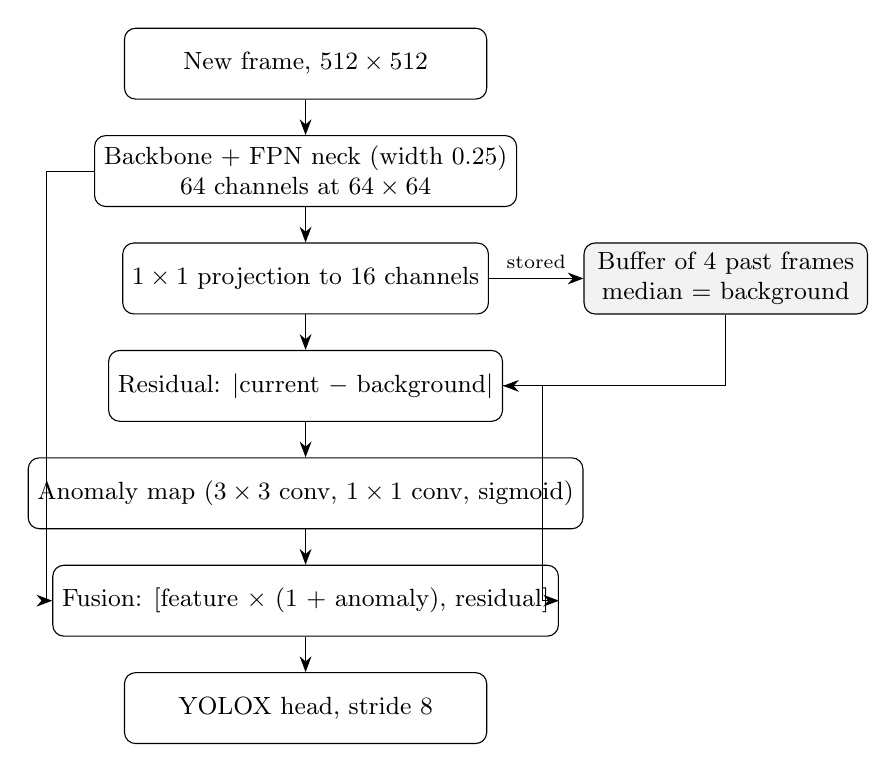
\begin{tikzpicture}[
  box/.style={draw, rounded corners, align=center, minimum width=4.6cm, minimum height=0.9cm, font=\small},
  side/.style={draw, rounded corners, align=center, minimum width=3.6cm, minimum height=0.9cm, font=\small, fill=gray!10},
  arr/.style={-{Stealth[length=2mm]}},
  node distance=0.45cm]
\node[box] (frame) {New frame, $512\times512$};
\node[box, below=of frame] (bb) {Backbone + FPN neck (width 0.25)\\64 channels at $64\times64$};
\node[box, below=of bb] (proj) {$1\times1$ projection to 16 channels};
\node[side, right=1.2cm of proj] (buf) {Buffer of 4 past frames\\median = background};
\node[box, below=of proj] (res) {Residual: $|$current $-$ background$|$};
\node[box, below=of res] (anom) {Anomaly map ($3\times3$ conv, $1\times1$ conv, sigmoid)};
\node[box, below=of anom] (fuse) {Fusion: [feature $\times$ (1 + anomaly), residual]};
\node[box, below=of fuse] (head) {YOLOX head, stride 8};
\draw[arr] (frame) -- (bb);
\draw[arr] (bb) -- (proj);
\draw[arr] (proj) -- (res);
\draw[arr] (proj) -- node[above, font=\scriptsize]{stored} (buf);
\draw[arr] (buf) |- (res);
\draw[arr] (res) -- (anom);
\draw[arr] (anom) -- (fuse);
\draw[arr] (fuse) -- (head);
\draw[arr] (bb.west) -- ++(-0.6,0) |- (fuse.west);
\draw[arr] (res.east) -- ++(0.5,0) |- (fuse.east);
\end{tikzpicture}
\caption{The student. Only the newest frame goes through the backbone; past frames are kept as 16-channel maps.}
\label{fig:student}
\end{figure}

\begin{table}[htbp]
\centering
\caption{Student blocks, for one new frame at $512\times512$.}
\label{tab:student}
\small
\begin{tabular}{llrr}
\toprule
Block & Output & Parameters & MACs \\
\midrule
Backbone (CSPDarknet, width 0.25, depth 0.33) & 64/128/256 ch at stride 8/16/32 & 1{,}056.7\,k & 0.950\,G \\
Neck (top-down FPN) & 64 ch, $64\times64$ & 155.1\,k & 0.207\,G \\
Projection ($1\times1$, 64 $\to$ 16) & 16 ch, $64\times64$ & 1.0\,k & 0.004\,G \\
Median background and residual & 16 ch, $64\times64$ & 0 & not counted \\
Anomaly map & 1 ch, $64\times64$ & 2.4\,k & 0.010\,G \\
Fusion ($3\times3$, 80 $\to$ 64) & 64 ch, $64\times64$ & 46.2\,k & 0.190\,G \\
YOLOX head & 6 ch, $64\times64$ & 152.6\,k & 0.628\,G \\
\midrule
Total & & 1{,}414\,k & 1.99\,G \\
\bottomrule
\end{tabular}
\end{table}

Running the student frame by frame gives the same output as running it on a full 5-frame clip (largest
difference $5\times10^{-8}$), so it can run live. At the start of a sequence the buffer is filled with the first
frame, which is also what the data loader does. The student is trained from scratch with AdamW, learning rate
$5\times10^{-4}$, cosine schedule and batch 4. Its objectness and class outputs start at 1\% probability, so it
does not have to unlearn a 50\% guess on every empty cell.

\section{The full proposed model}

\subsection{FDAM-style attention in the teacher}

FDAM~\cite{fdam} points out that attention acts like a low-pass filter. We added its two parts to CHAL's
spatio-temporal Swin transformer (one layer, 2 heads, 32 channels, windows of 5 frames $\times$ $4\times4$ pixels):
\begin{itemize}
  \item \textbf{Attention inversion.} If $A$ is the attention matrix, $I-A$ is the matching high-pass filter. For
        each token and head, the output becomes $(1+a)\,Av + b\,(v - Av)$, where $a$ and $b$ come from a small
        linear layer on the token.
  \item \textbf{Frequency scaling.} After the Swin layer, each frame's feature map is moved to the frequency domain
        with a 2-D FFT, split into $4\times4$ bands, and each band is scaled by a learned amount that depends on
        the frame.
\end{itemize}
Both parts start at zero, so the FDAM teacher starts out identical to the original one (we checked: outputs
matched to within $2\times10^{-6}$). FDAM adds 1{,}172 parameters. This is our own adaptation; the FDAM paper did
not test it on Swin-style window attention.

\subsection{Distillation}

All distilled students add one loss term that matches the student's final feature map to the teacher's feature
map just before its head (128 channels, $64\times64$, normalised per channel). A $1\times1$ layer maps the
student's 64 channels to 128. This layer is used only during training and is not part of the deployed student.

\begin{itemize}
  \item \textbf{Feature distillation (S1)} uses plain mean squared error.
  \item \textbf{Frequency-balanced distillation (S2, S3)} measures the same error in the frequency domain. The
        spectrum is split into 8 rings by frequency, and each ring is weighted by the inverse of the teacher's
        power in that ring. No ring can weigh more than 10 times the strongest ring, and the weights average to 1.
\end{itemize}
The reason for the weighting is that a plain squared error is dominated by low frequencies, where most of the
teacher's feature energy is. The weighting gives each ring a fair share. We did not assume that high frequencies
contain only targets, since edges and noise are there too, which is why the weights are capped. With equal
weights this loss is exactly the plain squared error, which we checked numerically. The 8 rings and the cap of 10
were fixed before training; they were not tuned, because our validation set could not tell close models apart
(Section~6).

\subsection{Configurations}

\begin{itemize}
  \item T0: original CHAL teacher. \quad T1: CHAL teacher with FDAM.
  \item S0: student, labels only.
  \item S1: student + feature distillation from T0.
  \item S2: student + frequency-balanced distillation from T0.
  \item S3 (full proposed model): student + frequency-balanced distillation from T1.
\end{itemize}
Both teachers were trained in the same Kaggle session with the same settings for 4 epochs. All four students were
trained in one session for 8 epochs. The number of epochs was chosen before training from the measured speed, so
everything fitted in our GPU budget. Each model was trained once.

\section{Results}

\subsection{Detection}

\begin{table}[htbp]
\centering
\caption{Test set, paper metrics (\%). The paper row uses the paper's own split, which may differ from ours.}
\label{tab:paper-metrics}
\begin{tabular}{lcccc}
\toprule
Model & mAP50 & Precision & Recall & F1 \\
\midrule
CHAL, paper & 75.25 & 86.35 & 88.49 & 87.41 \\
\midrule
T0: original teacher & 64.8 & 89.7 & 73.4 & 80.7 \\
T1: FDAM teacher & 60.6 & 87.4 & 70.3 & 77.9 \\
S0: labels only & 75.0 & 86.0 & 88.4 & 87.2 \\
S1: feature distillation & 73.2 & 86.0 & 86.3 & 86.1 \\
S2: frequency-balanced & 73.1 & 86.9 & 85.7 & 86.3 \\
S3: full model & 74.6 & 86.5 & 87.6 & 87.1 \\
\bottomrule
\end{tabular}
\end{table}

\begin{table}[htbp]
\centering
\caption{Test set, brief metrics, at the threshold chosen on validation.}
\label{tab:brief-metrics}
\begin{tabular}{lccccc}
\toprule
Model & Threshold & Pd (\%) & Precision (\%) & F1 (\%) & False alarms / frame \\
\midrule
T0 & 0.65 & 51.7 & 100.0 & 68.2 & 0.000 \\
T1 & 0.55 & 56.2 & 88.6 & 68.8 & 0.062 \\
S0 & 0.40 & 82.9 & 98.6 & 90.1 & 0.010 \\
S1 & 0.40 & 80.6 & 98.0 & 88.5 & 0.015 \\
S2 & 0.35 & 85.9 & 95.1 & 90.3 & 0.038 \\
S3 & 0.40 & 79.2 & 98.6 & 87.9 & 0.009 \\
\bottomrule
\end{tabular}
\end{table}

\begin{table}[htbp]
\centering
\caption{Low-contrast test sequences (8 sequences, 529 targets) and the background-change test.}
\label{tab:lowc-bg}
\begin{tabular}{lcccccc}
\toprule
 & \multicolumn{3}{c}{Low contrast} & Other & \multicolumn{2}{c}{Background change} \\
\cmidrule(lr){2-4}\cmidrule(lr){5-5}\cmidrule(lr){6-7}
Model & Pd (\%) & F1 (\%) & FA / frame & Pd (\%) & Pd (\%) & Pd change \\
\midrule
T0 & 11.5 & 20.7 & 0.000 & 69.4 & 49.4 & $-2.3$ \\
T1 & 15.7 & 22.6 & 0.152 & 74.1 & 52.3 & $-3.9$ \\
S0 & 59.0 & 72.9 & 0.019 & 93.4 & 77.6 & $-5.3$ \\
S1 & 57.5 & 71.1 & 0.028 & 90.8 & 76.7 & $-3.9$ \\
S2 & 67.1 & 76.3 & 0.059 & 94.3 & 82.7 & $-3.2$ \\
S3 & 50.1 & 65.4 & 0.020 & 92.1 & 74.1 & $-5.1$ \\
\bottomrule
\end{tabular}
\end{table}

\subsection{The controlled comparisons}

Because each model was trained once, we treat a difference of less than 2 points as no clear difference.

\begin{table}[htbp]
\centering
\caption{Differences between configurations on the test set (points; false alarms per frame).}
\label{tab:ablations}
\small
\begin{tabular}{lcccccl}
\toprule
Comparison & F1 & Pd & Pd low-c. & FA/frame & mAP50 & Reading \\
\midrule
T1 vs T0 (FDAM) & $+0.6$ & $+4.5$ & $+4.2$ & $+0.062$ & $-4.2$ & no clear gain \\
S1 vs S0 (distillation) & $-1.6$ & $-2.3$ & $-1.5$ & $+0.005$ & $-1.7$ & no gain \\
S2 vs S1 (frequency) & $+1.8$ & $+5.3$ & $+9.6$ & $+0.023$ & $-0.1$ & more found, more FA \\
S3 vs S2 (FDAM teacher) & $-2.4$ & $-6.7$ & $-17.0$ & $-0.029$ & $+1.4$ & worse \\
\bottomrule
\end{tabular}
\end{table}

\paragraph{FDAM teacher (T1 vs T0).} F1 is about the same. FDAM found more targets but also made more false
alarms, and its mAP50 was lower. Its learned FDAM weights stayed small after 4 epochs at the authors' learning
rate (frequency weights averaged 0.0007), so it may not have had time to use FDAM much.

\paragraph{Distillation (S1 vs S0).} Feature distillation did not help. Both teachers find only 52--56\% of test
targets, while the student alone finds 83\%. Copying a teacher that is weaker than the student seems to pull the
student towards the teacher's mistakes.

\paragraph{Frequency weighting (S2 vs S1).} The frequency-balanced loss found clearly more targets, mostly in
low-contrast sequences (67.1\% against 57.5\%, the best low-contrast result of all six models). It also made about
2.5 times as many false alarms, so F1 only rose by 1.8 points.

\paragraph{Full model (S3 vs S2).} Using the FDAM teacher instead of the original made the student worse, mainly
on low-contrast targets.

\paragraph{Background change.} All models lost some Pd. The students lost 3.2--5.3 points and the teachers
2.3--3.9. S2 lost the least among the students, but the differences are small for single runs. This test only
covers smooth brightness changes, and it does not show that any model has learned a causal relationship.

\paragraph{Validation.} The four students had almost the same validation F1 (90.5--91.2\%), while their test F1
ranged from 87.9 to 90.3\%. So our validation set could not rank close models, even with a low-contrast sequence
in it.

\subsection{Earlier pilot run}

Before freezing the split, we ran the student comparisons once on our earlier split. That split's validation had
no low-contrast sequence, the students trained for 17 epochs, and the teacher was the 50-epoch one. The pattern
was the same (Table~\ref{tab:pilot}). We re-ran the evaluation of the label-only student on a second machine and
got exactly the same numbers. The frequency student in the pilot used an earlier, simpler weighting (high
frequencies weighted 2$\times$), which we replaced after feedback from our TA.

\begin{table}[htbp]
\centering
\caption{Pilot on the earlier split (test set). Not directly comparable with Tables~\ref{tab:paper-metrics}--\ref{tab:lowc-bg}.}
\label{tab:pilot}
\small
\begin{tabular}{lcccccc}
\toprule
Model & F1 (\%) & Pd (\%) & Pd low-c. (\%) & FA / frame & mAP50 (\%) & COCO F1 (\%) \\
\midrule
Teacher, 50 epochs & 67.5 & 61.3 & 25.7 & 0.175 & 58.1 & 76.4 \\
Student, labels only & 93.5 & 91.8 & 78.4 & 0.040 & 78.1 & 89.0 \\
Student + feature distillation & 90.2 & 87.6 & 66.4 & 0.058 & 77.0 & 88.2 \\
Student + frequency (high $\times$2) & 88.0 & 91.1 & 74.1 & 0.138 & 79.0 & 89.7 \\
\bottomrule
\end{tabular}
\end{table}

\subsection{Size and speed}

All models were timed in the same session on the same laptop CPU (AMD Ryzen AI 7 350), with 32-bit weights, batch
1, and the input already in memory. We timed the model only (no image loading or NMS) and report the median of 30
runs. To be fair to the teacher, we also timed a version that keeps its backbone features from the past 4 frames,
so it only runs the backbone on the new frame.

\begin{table}[htbp]
\centering
\caption{Cost per new frame. MACs are counted with thop, which skips operations without weights (the median, FFTs).}
\label{tab:speed}
\small
\begin{tabular}{lccccc}
\toprule
Model & Parameters & GMACs & Buffer & 8 threads & 1 thread \\
\midrule
Teacher, recomputing 5 frames & 15.75\,M & 167.0 & 1.05\,MB & 908\,ms & 2{,}918\,ms \\
Teacher, caching past features & 15.75\,M & 117.0 & 14.7\,MB & 685\,ms & 2{,}030\,ms \\
FDAM teacher, recomputing & 15.75\,M & 167.0 & 1.05\,MB & 881\,ms & 2{,}907\,ms \\
FDAM teacher, caching & 15.75\,M & 117.0 & 14.7\,MB & 665\,ms & 2{,}030\,ms \\
Student & 1.41\,M & 1.99 & 1.05\,MB & 17.3\,ms & 46.9\,ms \\
\bottomrule
\end{tabular}
\end{table}

Caching only reduces the teacher's compute by 30\%, because most of its cost is in the neck, which still processes
all five frames. Even against the caching teacher, the student needs 59 times fewer MACs and is about 40 times
faster. The paper reports 137.04\,GFLOPs for CHAL, while we count 167\,GMACs at $512\times512$; we could not find
the reason for this difference. We did not measure energy, and we did not run anything on an edge device.

\section{Limitations}

\begin{itemize}
  \item \textbf{Weak teacher.} Our CHAL teachers are well below the published results. Likely reasons are our
        rebuilt CBAM module, the 920 untrained parameters, shorter training and possibly a different split. So
        our results say that distillation from \emph{our} CHAL teachers did not help; they do not show that
        distillation from a good CHAL model would not help.
  \item \textbf{Single, short runs.} Each configuration was trained once. Teachers trained for 4 epochs in the
        main comparison and students for 8. Most differences between students are close to what we would expect
        from run-to-run variation.
  \item \textbf{Comparison with the paper.} The label-only student scores close to the paper's CHAL on the paper's
        metric, but we cannot confirm the paper used the same test set, so this is not a fair head-to-head.
  \item \textbf{One dataset.} We only used NUDT-MIRSDT; the paper also uses DAUB-H and IRDST-R.
  \item \textbf{Validation.} Only one validation sequence counts as low-contrast by our measure, and validation
        did not separate the students. This is why we did not tune the frequency weighting.
  \item \textbf{Hardware.} Latency is from one laptop CPU only. Energy and edge-device results are missing.
  \item \textbf{Robustness.} The background-change test only uses smooth brightness patterns away from the target.
\end{itemize}

\section{Conclusion}

What worked: we built a compact student that is about 11 times smaller and about 40 times faster than CHAL on a
CPU, and on our split it detected far more targets than our retrained CHAL teachers. We also froze an evaluation
setup, ran matched comparisons, and found several bugs, including one in CHAL's public training code.

What did not work: our CHAL reproduction stayed well below the paper. Because of this, feature distillation from
it did not help the student, and the FDAM teacher did not become clearly better. Frequency-balanced distillation
was the most promising variant, since it found more low-contrast targets, but it also raised false alarms and
needs repeated runs before we can trust it.

The most useful next steps are to find out why the teacher is weak (for example, train the missed parameters and
try a higher learning rate), repeat the close comparisons with more seeds, and test the student on the other two
datasets.

\begin{thebibliography}{9}

\bibitem{chal}
W.~Duan, L.~Ji, S.~Lei, S.~Zhu, J.~Huang and M.~Ye.
CHAL: Causal-guided Hierarchical Anomaly-aware Learning for Moving Infrared Small Target Detection.
In \emph{CVPR}, pp.~21357--21366, 2026.
Code: \url{https://github.com/UESTC-nnLab/CHAL}

\bibitem{fdam}
L.~Chen, L.~Gu and Y.~Fu.
Frequency-Dynamic Attention Modulation for Dense Prediction.
In \emph{ICCV}, pp.~22620--22632, 2025.
Code: \url{https://github.com/Linwei-Chen/FDAM}

\bibitem{sdkd}
Y.~Li, C.~Yang, H.~Zeng, Z.~Dong, Z.~An, Y.~Xu, Y.~Tian and H.~Wu.
Frequency-Aligned Knowledge Distillation for Lightweight Spatiotemporal Forecasting.
In \emph{ICCV}, pp.~7262--7272, 2025.
Code: \url{https://github.com/itsnotacie/SDKD}

\end{thebibliography}

\end{document}
